\documentclass[12pt, letterpaper]{article}
\usepackage[utf8]{inputenc}
\usepackage{amsmath}
\usepackage{changepage}% http://ctan.org/pkg/changepage
\usepackage{titlesec} 
\usepackage{placeins}
\usepackage{caption}
\newcommand\tab[1][1cm]{\hspace*{#1}}
\titleformat{\subsection}[runin]{}{}{}{}[]
\usepackage{graphicx}


\title{CS M148 Homework 3}
\author{Hanna Co}
\date{Due: February 25, 2022}

\begin{document}
\maketitle
\newpage
\section{Multinomial Logistic Regression}
\subsection*{a)} Given $ln\frac{P(Y_i=1)}{P(Y_i=K)} = \beta_iX_i$, we can derive the probability for the event that $Y_i=1$:\\
$\frac{P(Y_i=1)}{P(Y_i=K)}=e^{\beta_iX_i}$\\
$P(Y_i=1)=P(Y_I=K)e^{\beta_iX_i}$\\
Since we know the sum of all probabilities must add up to 1:\\
$K*P(Y_i=K)\sum_{i=1}^{K}e^{\beta_iX_i}=1$\\
Thus, we can derive the probability for $P(Y_i=K)$:\\
$P(Y_i=K)=\frac{1}{K\sum_{i=1}^{K}e^{\beta_iX_i}}$

\subsection*{b)} TODO

\newpage
\section{Decision Trees}
\subsection*{a)} We first begin by calculating entropy values for the table, and for each split:\\
Total Entropy: $-\frac{5}{11}log_2\frac{5}{11}-\frac{6}{11}log_2\frac{6}{11}=0.994$\\\\
 \begin{tabular}{ |c|c|c|c|c|c|c| } 
 \hline
 \textbf{Feature} & \textbf{Left} & \textbf{Right}& \textbf{Entropy(L)}& \textbf{Entropy(R)}& \textbf{Weighted Avg}& \textbf{Info Gain} \\ 
\hline
Price & \$ & \$\$,\$\$\$ & 0.918 & 0.954 & 0.945 & 0.049 \\ 
\hline
Price & \$\$& \$,\$\$\$ & 0.971 & 0.918 & 0.942 & 0.052 \\ 
\hline
Price & \$\$\$& \$,\$\$ & 0 & 0.99 & 0.811 & 0.183 \\ 
 \hline
Location & LA & LB, B & 0.918 & 1 & 0.978 & 0.016 \\ 
 \hline
Location & B & LA,  LB & 1 & 0.985 & 0.991 & 0.003 \\ 
 \hline
Location & LB & LA, B & 1 & 0.985 & 0.991 & 0.003 \\ 
 \hline
Level & B & I, A & 0.918 & 0.954 & 0.945 & 0.049 \\ 
 \hline
Level & I & B, A & 1 & 0.985 & 0.991 & 0.003 \\ 
 \hline
Level & A & I, B & 0.918 & 1 & 0.978 & 0.016 \\ 
 \hline
Type & F & T, B & 0.918 & 1 & 0.978 & 0.016 \\ 
 \hline
Type & T & F, B & 0.918 & 0.954 & 0.945 & 0.049 \\ 
 \hline
Type & B & T, F & 0.971 & 1 & 0.987 & 0.007 \\ 
 \hline
\end{tabular}\\\\
Splitting on \{\{\$\$\$\}, \{\$, \$\$\}\} gives us the largest information gain, so we split on that feature, and recalculate our entropy values.\\\\
Total Entropy: $-\frac{5}{9}log_2\frac{5}{9}-\frac{6}{9}log_2\frac{6}{9}=0.861$\\\\
 \begin{tabular}{ |c|c|c|c|c|c|c| } 
 \hline
 \textbf{Feature} & \textbf{Left} & \textbf{Right}& \textbf{Entropy(L)}& \textbf{Entropy(R)}& \textbf{Weighted Avg}& \textbf{Info Gain} \\ 
\hline
Price & \$ & \$\$ & 1 & 0.971 & 0.984 & 0.007 \\ 
 \hline
Location & LA & LB, B & 1 & 0.985 & 0.989 & 0.003 \\ 
 \hline
Location & B & LA,  LB & 1 & 0.971 & 0.984 & 0.009 \\ 
 \hline
Location & LB & LA, B & 0.918 & 1 & 0.973 & 0.018 \\ 
 \hline
Level & B & I, A & 0.918 & 1 & 0.973 & 0.018 \\ 
 \hline
Level & I & B, A & 0.918 & 1 & 0.973 & 0.018 \\ 
 \hline
Level & A & I, B & 0.918 & 0.918 & 0.918 & 0.073 \\ 
 \hline
Type & F & T, B & 1 & 0.985 & 0.988 & 0.003 \\ 
 \hline
Type & T & F, B & 0.918 & 1 & 0.973 & 0.018 \\ 
 \hline
Type & B & T, F & 1 & 0.971 & 0.934 & 0.007 \\ 
 \hline
\end{tabular}\\\\
This time, splitting on \{\{Advanced, \{Beginner, Intermediate\}\} gives us the largest information gain, so we split on that feature, and again recalculate.\\\\
Total Entropy: $-\frac{2}{6}log_2\frac{2}{6}-\frac{4}{6}log_2\frac{4}{6}=0.918$\\\\
 \begin{tabular}{ |c|c|c|c|c|c|c| } 
 \hline
 \textbf{Feature} & \textbf{Left} & \textbf{Right}& \textbf{Entropy(L)}& \textbf{Entropy(R)}& \textbf{Weighted Avg}& \textbf{Info Gain} \\ 
\hline
Price & \$ & \$\$ & 0.918 & 0.918 & 0.918 & 0 \\ 
 \hline
Location & LA & LB, B & 1 & 0.811 & 0.874 & 0.044 \\ 
 \hline
Location & B & LA,  LB & 0.918 & 0.918 & 0.918 & 0 \\ 
 \hline
Location & LB & LA, B & 0 & 0.971 & 0.809 & 0.109 \\ 
 \hline
Level & I & B & 0.918 & 0.918 & 0.918 & 0 \\ 
 \hline
Type & F & T, B & 1 & 0.811 & 0.874 & 0.044 \\ 
 \hline
Type & T & F, B & 0 & 1 & 0.667 & 0.251 \\ 
 \hline
Type & B & T, F & 1 & 0.811 & 0.874 & 0.044 \\ 
 \hline
\end{tabular}\\\\
Splitting on \{\{Tennis\}, \{Football, Basketball\}\} gives us the largest entropy gain, so we split on that.
TODO

\subsection*{b)} TODO

\subsection*{c)} TODO

\subsection*{d)} TODO

\subsection*{e)} TODO


\newpage
\section{Decision Tree (Short Answers)}
\subsection*{a)} It's more likely to overfit on non-linearly separable data on the left. This is because not being linearly separable can be indicative of many features that differentiate the two classes. The tree would try to account for all of these and overfit. Instead, I would use a logistic regression model.

\subsection*{b)}There is no need to standardize our data, as decision trees aren't sensitive to the magnitude of variables.

\subsection*{c)}Yes, decision trees are robust to outliers. This is because we split on certain values, such as being greater or less than some value. For example, say we have [1, 2, 3, 1000], and we split on 2. The fact that we have 1000 as an outlier doesn't affect our results.

\newpage
\section{Random Forest}
\subsection*{a)} $R^2=0.664$
\begin{figure}[h!]
  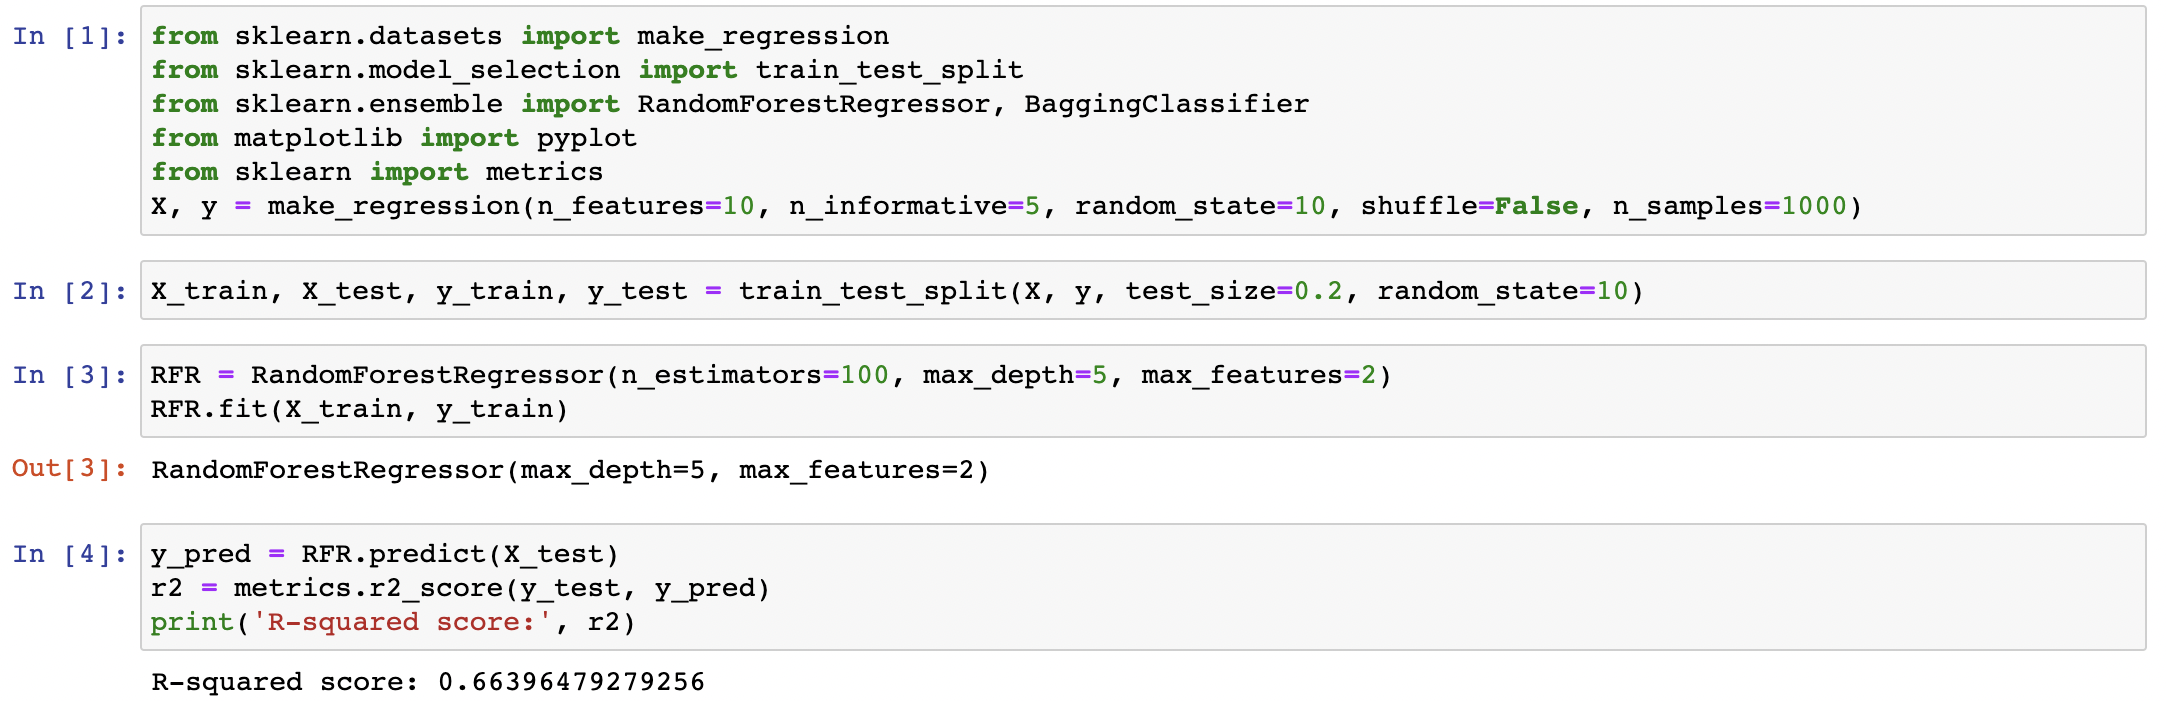
\includegraphics[scale=0.4]{./images/4a}
\end{figure}

\subsection*{b)}I would increase the depth and increase the number of features we split on. After playing around with these parameters, the ones that produced the best results for me were max\_depth=12 and max\_features=5, giving and $R^2$ value of 0.913.\\
\begin{figure}[h!]
  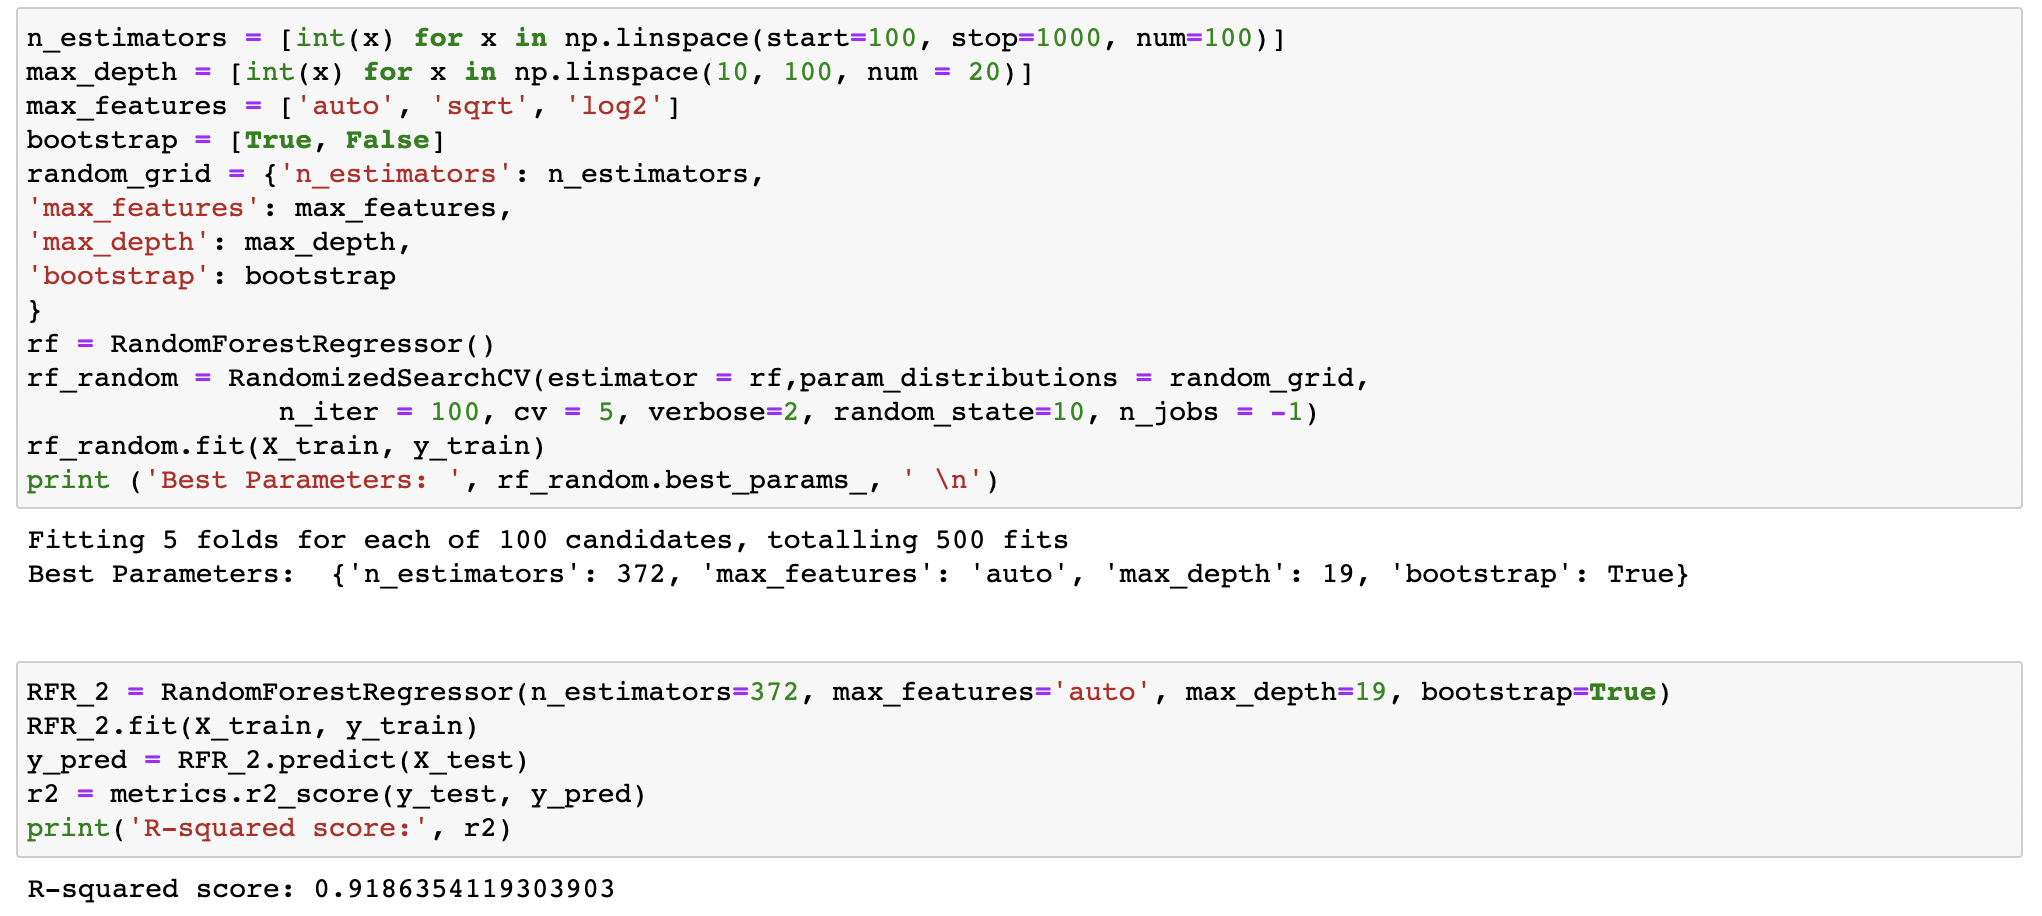
\includegraphics[scale=0.4]{./images/4b}
\end{figure}

\subsection*{c)} Variable Importance
\begin{figure}[h!]
  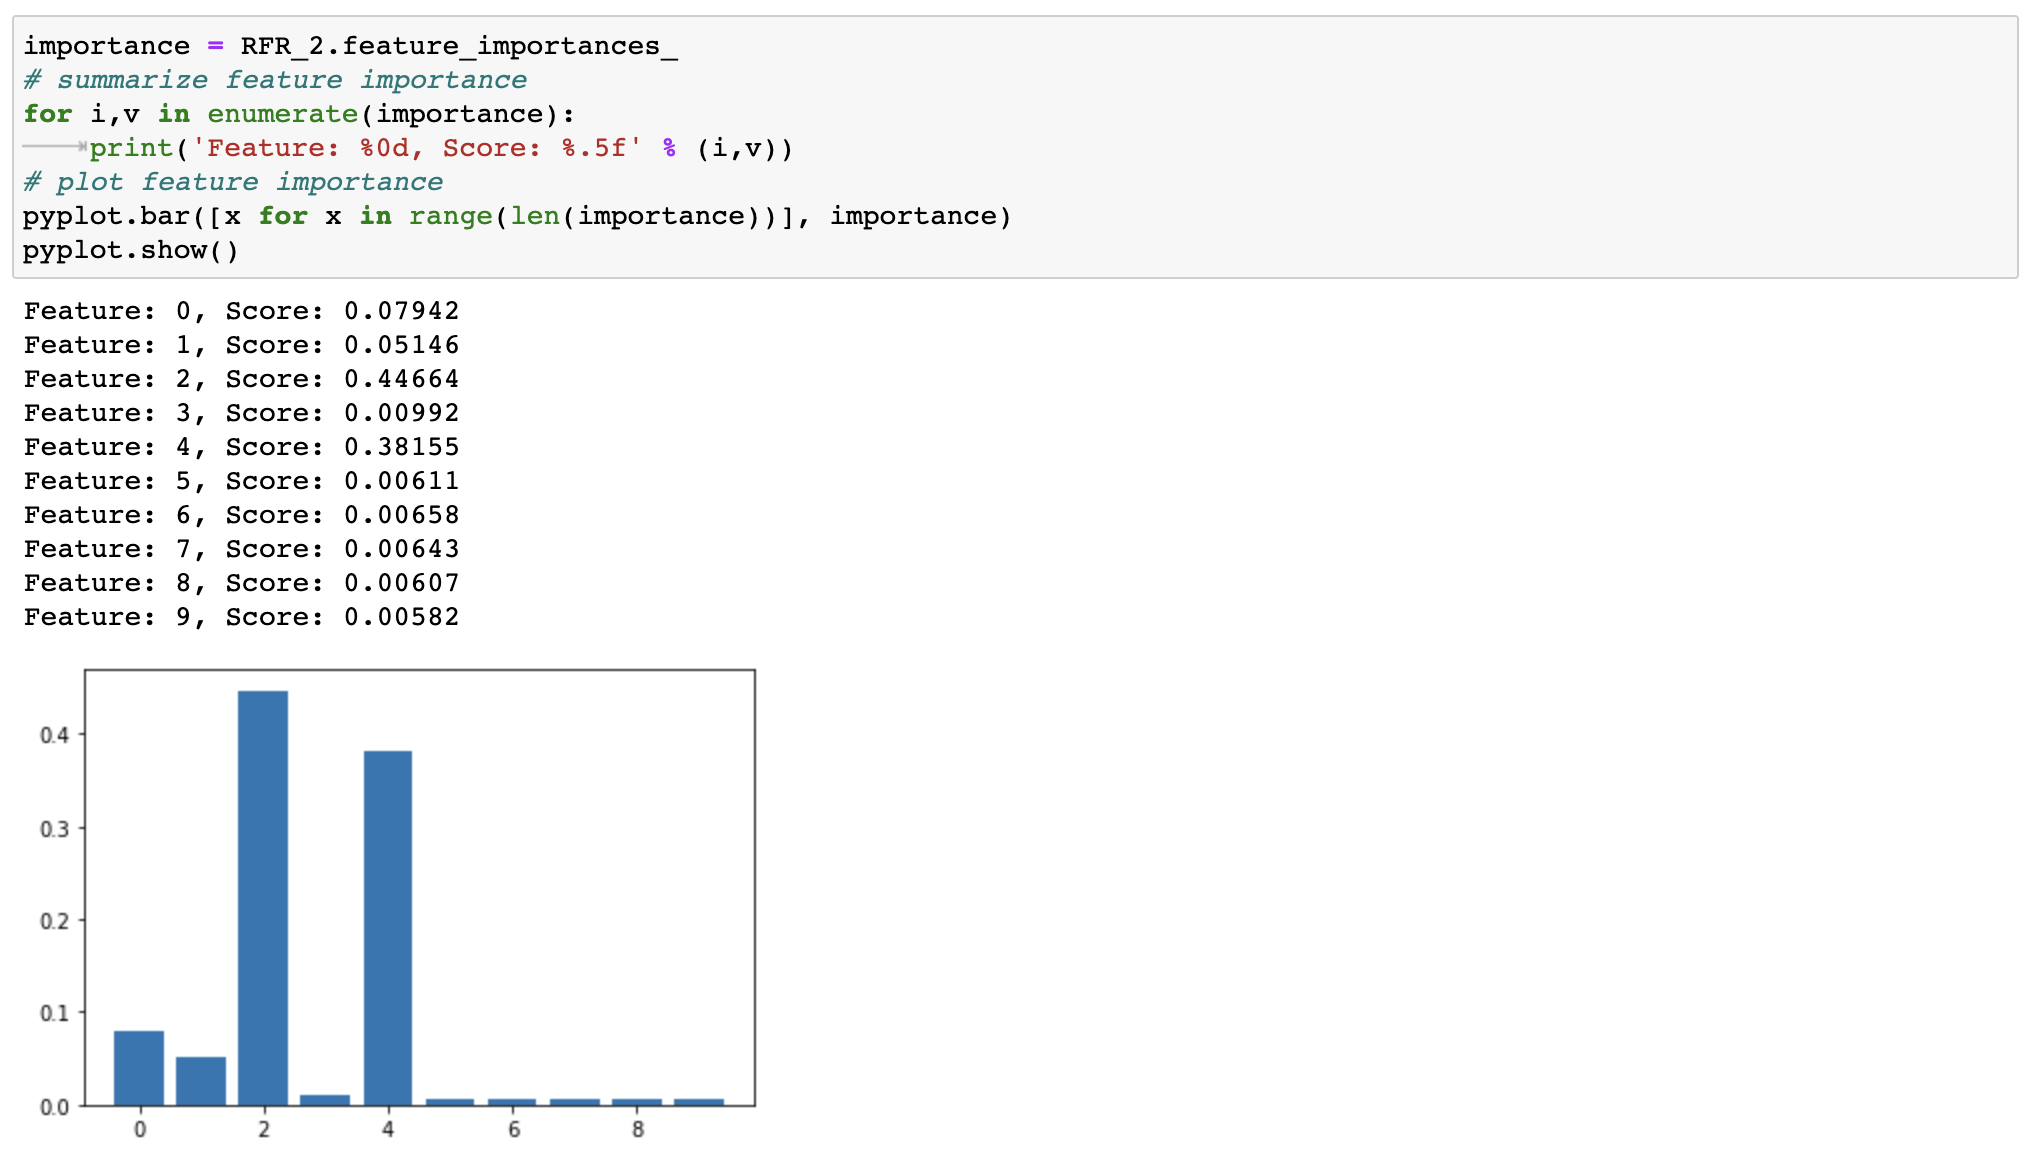
\includegraphics[scale=0.4]{./images/4c}
\end{figure}
\clearpage

\subsection*{d)} Using the same parameters, the feature importance for the two models are nearly identical.
\begin{figure}[h!]
  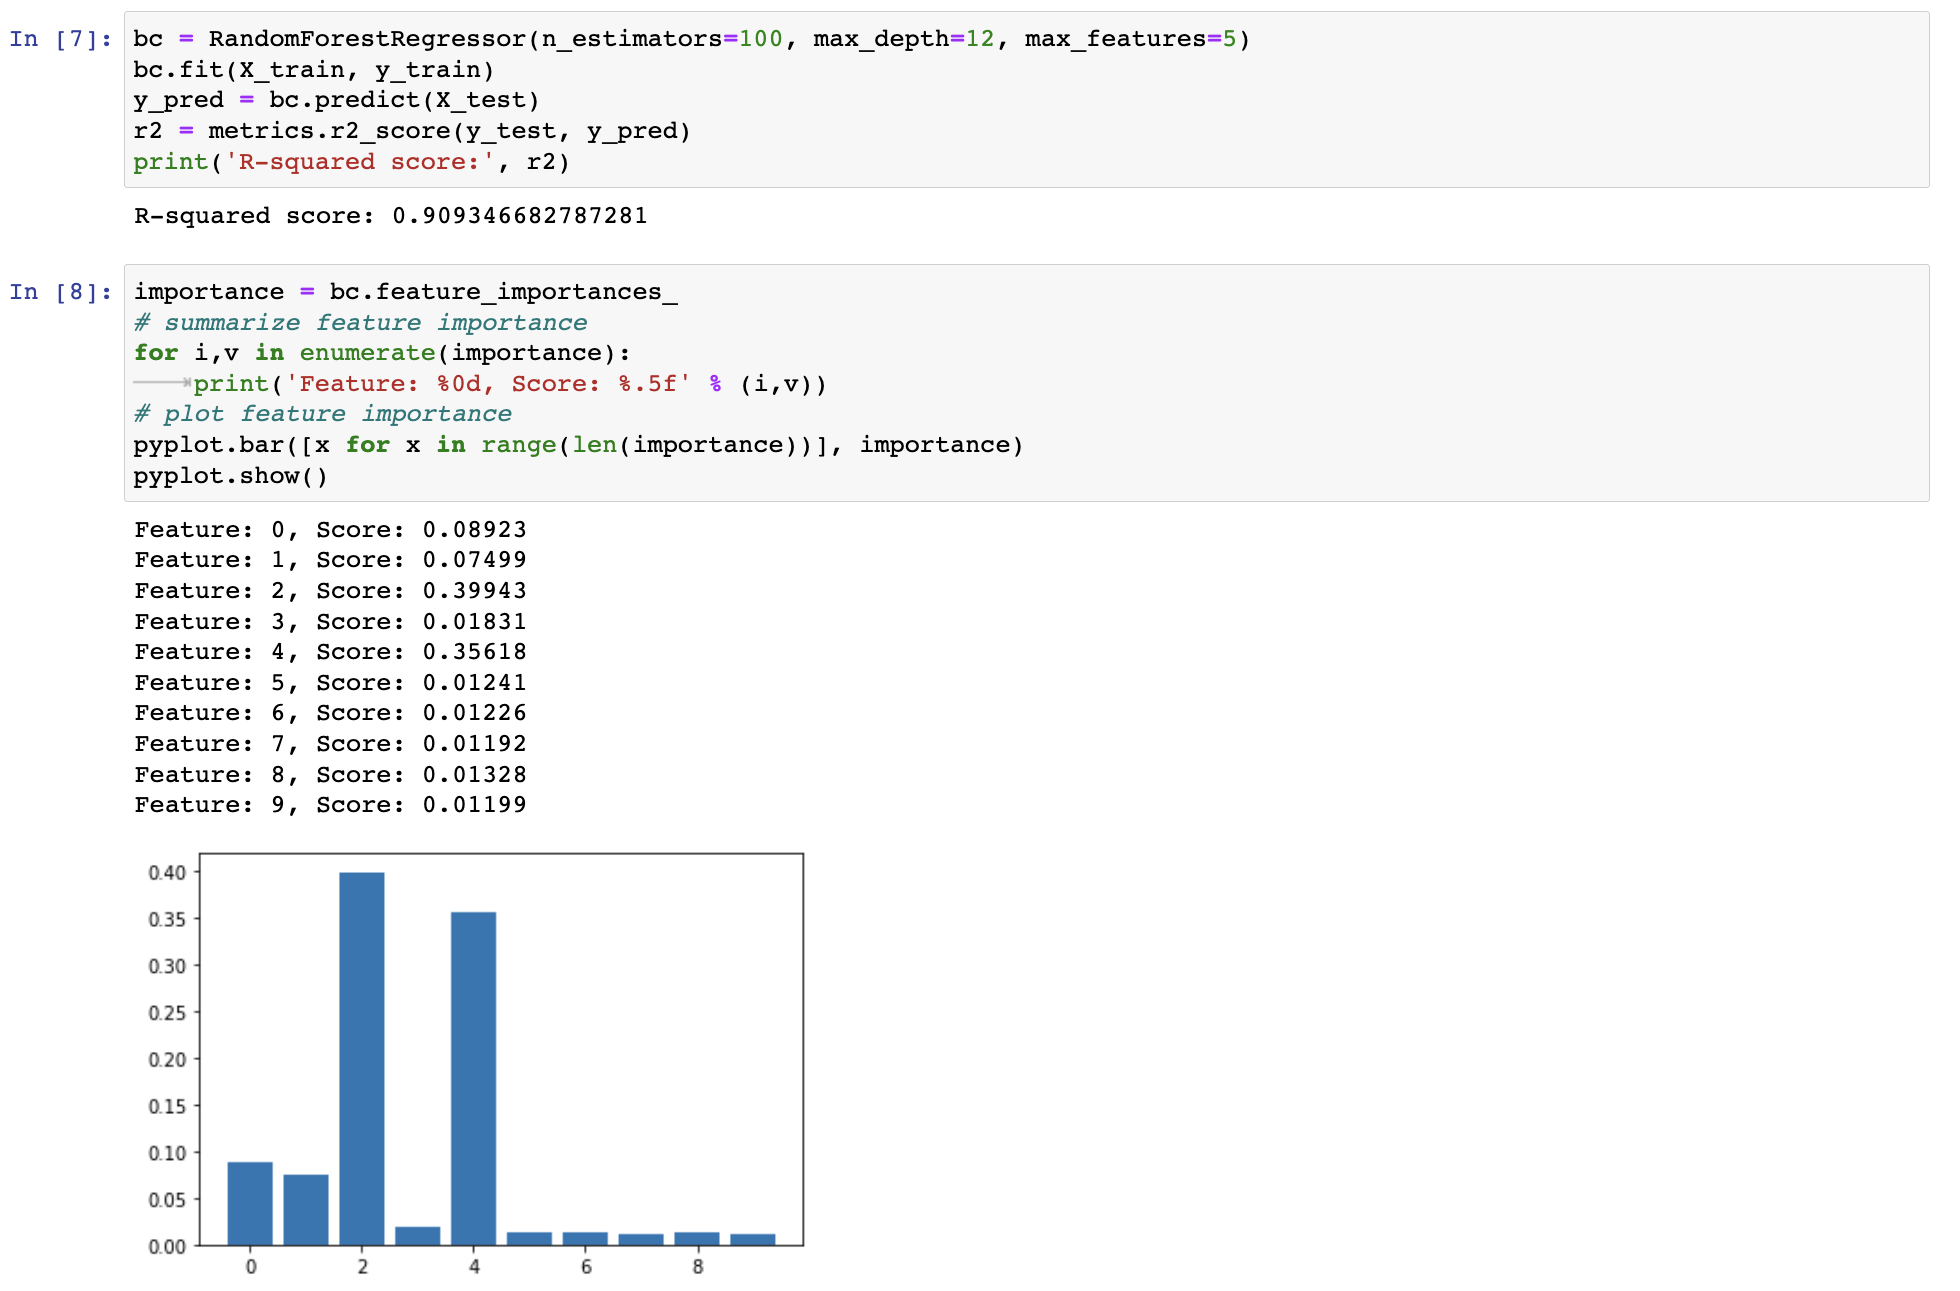
\includegraphics[scale=0.4]{./images/4d}
\end{figure}
\clearpage

\newpage
\section{Perceptron}
\subsection*{a)} $\Delta w_i=x(t-z)*x_i$\\
We are given that $w_1 = w_2 = b = 1$, and $c=2$\\
For the point $(2,-3)$, we can calculate $(2)(1)+(-3)(1)+1 = 0 \Rightarrow 0$\\
Since this does not match our predicted value, we must re-calculate our weights.\\
$\Delta w_1 = 2(1-0)*2 = 4 \Rightarrow w_1 = 1 + 4 = 5$\\
$\Delta w_2 = 2(1-0)*(-3) = -6 \Rightarrow w_2 = 1 - 6 = -5$\\
$\Delta b = 2(1-0)*1 = 2 \Rightarrow b = 1 + 2 = 3$\\
We now make a prediction for our next point, $(4, 4): (4)(5)+(4)(-5)+3 = 3 \Rightarrow 1$\\
Again, this does not match our predicted value, so we mush recalculate our weights.\\
$\Delta w_1 = 2(0-1)*4 = -8 \Rightarrow w_1 = 5 - 8 = -3$\\
$\Delta w_2 = 2(0-1)*4 = -8 \Rightarrow w_2 = -5 - 8 = -13$\\
$\Delta b = 2(0-1)*3 = -6 \Rightarrow b = 3 - 6 = -3$\\
We finally make a prediction for our last point, $(2, -3): (2)(-3)+(-3)(-13)-3 = 30 \Rightarrow 1$\\
This also doesn't match our actual value, so we adjust our weights one last time:\\
$\Delta w_1 = 2(0-1)*2 = -4 \Rightarrow w_1 = -3 - 4 = -7$\\
$\Delta w_2 = 2(0-1)*(-3) = 6 \Rightarrow w_2 = -13 + 6 = -5$\\
$\Delta b = 2(0-1)*(-3) = 6 \Rightarrow b = -3 + 6 = 3$\\

\subsection*{b)} It hasn't converged, because it is still mis-classifying points in our data. In this case, I don't expect it to converge, because (2, -3) has both 0 and 1 as actual values, which will continue to confuse our model.

\newpage
\section{ Neural Networks}
\subsection*{a)} Say we have $w_1=w_2=-1$, and $b = 1$. This will give us the following predictions:\\
$(0)(-1)+(0)(-1)+1 = 1 \Rightarrow +1$\\
$(0)(-1)+(1)(-1)+1 = 0 \Rightarrow +1$\\
$(1)(-1)+(0)(-1)+1 = 0 \Rightarrow +1$\\
$(1)(-1)+(1)(-1)+1 = -1 \Rightarrow -1$\\
As we can see, our data can be perfectly classfied with a single activation unit.\\

\subsection*{b)} As we can see from plotting the points, the data is no linearly separable, thus we can not perfectly classify it with a single activation unit.
\begin{figure}[h!]
  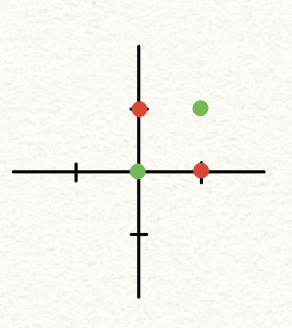
\includegraphics[scale=0.4]{./images/6b.jpeg}
\end{figure}
\clearpage

\subsection*{c)}Yes, you should be able to, by first separating (1, 1) from the other three points, then separating (0, 0) from the other three points. These two activation units and their weights can be combined to form a neural network that perfectly classifies these points.


\end{document}